% 第 9 章 领域特定语言
\renewcommand{\codeInset}{63bp}
前几章我们用 Qt 库开发了奥赛罗棋和圈叉棋两种游戏。本章我们将开始开发一种领域特定语言（Domain-Specific Language，DSL），即面向特定领域的语言。更具体地说，我们要开发一种在 Qt 部件中书写图形对象的语言。这门语言允许我们绘制直线、矩形、椭圆，并书写文本。此外，它还允许我们为图形对象选择颜色、笔样式和刷样式，也允许我们为文本选择字体和对齐方式。

本章将涵盖以下主题：

\begin{itemize}
\item 首先，我们通过一个示例来非正式地了解 DSL 的源代码。我们绘制图形对象，并设置它们的颜色、样式与字体。
\item 我们用文法形式化地定义这门语言。
\item 定义好文法之后，我们编写扫描器。扫描器读取源代码，识别出有意义字符序列，即词法单元（token）。
\item 扫描器写好后，我们编写解析器。解析器可以看作 DSL 的核心，它在需要时向扫描器请求新的词法单元；它检查源代码是否符合文法，并生成一个动作序列。每个动作持有一条指令，如设置颜色或绘制直线。
\item 最后，我们编写一个查看器：它读取解析器生成的动作序列，并在 Qt 部件中显示图形对象。
\end{itemize}

\section{引入源语言 —— 一个简单示例}

DSL 的源语言由一系列指令构成。既有绘制直线、矩形、椭圆和文本等图形对象的指令，也有设置对象颜色与样式、文本字体与对齐方式的指令。最后，还有为名字赋值的指令。

我们来看一个示例。下面的代码绘制一个矩形并书写文本。注意，这门语言区分大小写——也就是说，代码中用小写还是大写字母并无关系。我们先定义矩形的左上角：

\begin{codebox}
topLeft = point(100, 100);
\end{codebox}

我们用坐标运算符提取左上角点的 x 和 y 坐标，并定义右下角：

\begin{codebox}
left = xCoordinate(topLeft);
top = yCoordinate(topLeft);
bottomRight = point(left + 100, top + 100);
\end{codebox}

我们用预定义值 DashLine 和 CrossPattern 来设置笔和刷的样式：

\begin{codebox}
SetPenStyle(DashLine);
SetBrushStyle(CrossPattern);
\end{codebox}

我们把预定义颜色 Black 用作笔的颜色，并为刷创建一个自己的颜色 Purple。我们可以用三个值——分别对应红、绿、蓝分量——来创建一种新颜色。每个分量的取值范围为 0 到 255（含两端）：

\begin{codebox}
SetPenColor(Black);
PurpleColor = color(128, 0, 128);
SetBrushColor(PurpleColor);
DrawRectangle(topLeft, bottomRight);
\end{codebox}

我们接着添加一段文本，并设置字体和对齐方式。我们选用 12 磅的 Times New Roman、水平左对齐和垂直顶端对齐：

\begin{codebox}
SetFont(font("Times New Roman", 12));
SetHorizontalAlignment(AlignLeft);
SetVerticalAlignment(AlignTop);
DrawText(point(300, 150), "Hello, DSL!");
\end{codebox}

本示例中的指令会被扫描器切分成有意义的部分；解析器将检查指令是否符合文法，并生成一个动作序列，查看器读取该序列后显示以下 Qt 部件：

\begin{center}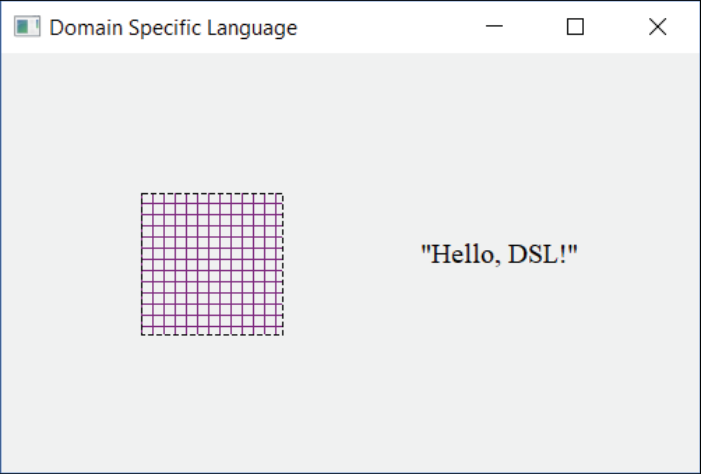
\includegraphics[width=235.4bp]{images/p365_i03.png}\end{center}

\subsection{源语言的文法}

DSL 的源语言需要被精确定义，我们通过定义该语言的文法来做到这一点。文法由规则（以斜体显示）、关键字（以粗体显示）、分隔符和标点符号构成。

程序规则是开始规则。箭头（\texttt{->}）表示一个程序由指令列表构成。该箭头可以读作：

\begin{codebox}
program -> instructionList
\end{codebox}

在文法中，星号（\texttt{*}）表示零个或多个。因此，指令列表由零条或多条指令构成：

\begin{codebox}
instructionList -> instruction*
\end{codebox}

赋值指令接受一个名字，后跟赋值运算符（\texttt{=}）、一个表达式和一个分号。设置笔和刷颜色与样式的指令接受一个表达式，设置字体和对齐方式的指令也是如此。绘制直线、矩形和文本的指令接受两个表达式。注意，每条指令都以分号（\texttt{;}）结尾。

竖线（\texttt{|}）可以读作「或」。一条指令就是一次赋值，或者设置笔的颜色，或者设置刷的颜色，如此等等：

\begin{codebox}
instruction -> name = expression;
             | SetPenColor(expression);
             | SetPenStyle(expression);
             | SetBrushColor(expression);
             | SetBrushStyle(expression);
             | SetFont(expression);
             | SetHorizontalAlignment(expression);
             | SetVerticalAlignment(expression);
             | DrawLine(expression, expression);
             | DrawRectangle(expression, expression);
             | DrawEllipse(expression, expression);
             | DrawText(expression, expression);
\end{codebox}

解析器接下来要定义的是表达式。我们先看表达式的运算符，还要考虑运算符的优先级。例如，乘法与除法的优先级高于加法与减法。文法中的运算符具有以下优先级：

\noindent\fontsize{10.5bp}{12bp}\selectfont
\setlength{\tabcolsep}{3.2bp}%
\renewcommand{\arraystretch}{1.07}%
\setlength{\extrarowheight}{5.4bp}%
\setlength{\arrayrulewidth}{0.4bp}%
\begin{tabular}{|p{108.3bp}|p{71.7bp}|p{36.4bp}|}
\hline
\textbf{表达式} & \textbf{运算符} & \textbf{优先级} \\
\hline
加法、减法 & {\ttfamily + -} & 最低 \\
\hline
乘法、除法 & {\ttfamily * /} & \\
\hline
\multicolumn{1}{|p{108.3bp}|}{\raisebox{-41.4bp}[0pt][0pt]{基本表达式}}%
 & {\ttfamily\fontsize{10bp}{12bp}\selectfont point\newline xCoordinate\newline yCoordinate\newline color\newline font\newline (expression)\newline name\newline value}%
 & \multicolumn{1}{p{36.4bp}|}{\raisebox{-41.4bp}[0pt][0pt]{最高}} \\
\hline
\end{tabular}

我们为加法与减法、乘法与除法各定义两条规则。先从最低的优先级入手，即加法与减法。在 \texttt{expression} 规则中，我们调用处理乘除表达式的 \texttt{mulDivExpression} 规则，并调用 \texttt{expressionRest} 规则来检查表达式的其余部分：

\begin{codebox}
expression -> mulDivExpression expressionRest
\end{codebox}

在 \texttt{expressionRest} 规则中，我们检查下一个词法单元。如果它是加号或减号，就得到一个加法或减法表达式。我们调用 \texttt{mulDivExpression} 来处理优先级更高的表达式。最后，如果又遇到一个加号或减号，就再次调用 \texttt{expressionRest}。不过，如果第一个词法单元既不是加号也不是减号，我们什么也不做：

\begin{codebox}
expressionRest -> + mulDivExpression expressionRest
                | - mulDivExpression expressionRest
                | /* empty */
\end{codebox}

\texttt{mulDivExpression} 与 \texttt{mulDivExpressionRest} 的工作方式与前面给出的 \texttt{expression} 和 \texttt{expressionRest} 相同：

\begin{codebox}
mulDivExpression -> primaryExpression mulDivExpressionRest
mulDivExpressionRest -> * primaryExpression mulDivExpressionRest
                      | / primaryExpression mulDivExpressionRest
                      | /* empty */
\end{codebox}

基本表达式可以是一个点、x 或 y 坐标、颜色、字体、名字或值。点由两个表达式构成，分别存放该点的 x 和 y 坐标。坐标接受一个存放点的表达式，并给出它的 x 或 y 坐标：

\begin{codebox}
primaryExpression -> point(expression, expression)
                   | xCoordinate(expression)
                   | yCoordinate(expression)
\end{codebox}

颜色表达式由其红、绿、蓝分量构成，而字体表达式由字体的名称和大小构成：

\begin{codebox}
                   | color(expression, expression, expression)
                   | font(expression, expression)
\end{codebox}

表达式可以括在圆括号中，以改变表达式的优先级。例如，在表达式 \texttt{2 + 3 * 4} 中，乘法优先于加法；而在表达式 \texttt{(2 + 3) * 4} 中，加法优先于乘法：

\begin{codebox}
                   | (expression)
\end{codebox}

最后，一个表达式可以是一个此前已与某个值关联的名字，或者干脆就是一个值：

\begin{codebox}
                   | name
                   | value
\end{codebox}

\subsection{目标语言}

目标语言由一系列动作定义。通俗地说，动作对应于文法中的指令。既有设置笔或刷的颜色与样式的动作，也有设置文本水平或垂直对齐方式的动作，还有真正绘制图形中的直线、矩形、椭圆和文本的动作。本章后面我们会编写一个解析器来生成动作序列，再编写一个查看器来读取这些动作，并在 Qt 部件中显示图形对象。

一个 \texttt{Action} 对象存放动作的标识（由 \texttt{Token} 类中的 \texttt{TokenId} 枚举定义如下），以及至多两个值。

\medskip\noindent{\ttfamily\bfseries Action.h}

\begin{codebox}
#ifndef ACTION_H
#define ACTION_H

#include "Token.h"
#include "Value.h"

class Action {
  public:
    Action(TokenId actionId, const Value& value1 = Value(),
           const Value& value2 = Value());
    Action(const Action& action);
    Action operator=(const Action& action);

    TokenId id() const {return m_actionId;}
    const Value& value1() const {return m_value1;}
    const Value& value2() const {return m_value2;}

  private:
    TokenId m_actionId;
    Value m_value1, m_value2;
};

#endif // ACTION_H
\end{codebox}

Action.cpp 文件存放 \texttt{Action} 类各方法的定义。

\medskip\noindent{\ttfamily\bfseries Action.cpp}

\begin{codebox}
#include "Action.h"
\end{codebox}

构造函数接受动作标识和至多两个值：

\begin{codebox}
Action::Action(TokenId actionId,
               const Value& value1 /*= Value()*/,
               const Value& value2 /*= Value()*/ )
  :m_actionId(actionId),
   m_value1(value1),
   m_value2(value2) {
  // Empty.
}
\end{codebox}

\subsection{颜色}

设置笔或刷的颜色时，我们需要随指令提交颜色。我们可以用前面文法中的 \texttt{color} 规则创建自己的颜色。不过，Qt 的 \texttt{QColor} 类提供了一组预定义颜色。下面的扫描器定义了一组预定义 \texttt{QColor} 对象（Aqua、Black 等），并把它们映射到各自的名称。例如，用户可以在源代码中写出如下指令：

\begin{codebox}
SetPenColor(Aqua);
\end{codebox}

此时，由于名称 \texttt{Aqua} 与 \texttt{QColor} 对象 \texttt{Aqua} 相关联，笔的颜色就被设置为 Aqua。

\medskip\noindent{\ttfamily\bfseries Colors.h}

\begin{codebox}
#ifndef COLOR_H
#define COLOR_H

#include <QWidget>

extern QColor
  Aqua, Black, Blue, Brown, Cyan, Gray, Green, Lime, Magenta,
  Navyblue, Orange, Orchid, Pink, Purple, Red, Silver, Snow,
  SteelBlue, SystemColor, Turquoise, Violet, White, Yellow;

#endif // COLOR_H
\end{codebox}

Colors.cpp 文件存放 Colors.h 中各颜色的定义。

\medskip\noindent{\ttfamily\bfseries Colors.cpp}

\begin{codebox}
#include "Colors.h"
\end{codebox}

每种颜色由其红、绿、蓝分量定义。每个分量的取值范围为 0 到 255（含两端）。例如，Blue 的蓝色分量取满值，其余分量为零；而 Yellow 是红与绿的混合：

\begin{codebox}
QColor
  Aqua(0, 255, 255), Black(0, 0, 0), Blue(0, 0, 255),
  Brown(165, 42, 42), Cyan(0, 255, 255), Gray(127, 127, 127),
  Green(0, 128, 0), Lime(0, 255, 0), Magenta(255, 0, 255),
  Navyblue(159, 175, 223), Orange(255, 165, 0),
  Orchid(218, 112, 214), Pink(255, 192, 203),
  Purple(128, 0, 128), Red(255, 0, 0), Silver(192, 192, 192),
  Snow(255, 250, 250), SteelBlue(70, 130, 180),
  SystemColor(0, 0, 0), Turquoise(64, 224, 208),
  Violet(238, 130, 238), White(255, 255, 255),
  Yellow(255, 255, 0);
\end{codebox}

\subsection{错误处理}

有几个用于错误处理的函数：\texttt{check} 检查某个条件是否为真，若不为真则报告错误；\texttt{syntaxError} 与 \texttt{semanticError} 分别报告语法错误和语义错误，而 \texttt{error} 抛出异常，由 \texttt{main} 函数捕获并报告。

\medskip\noindent{\ttfamily\bfseries Error.h}

\begin{codebox}
#ifndef ERROR_H
#define ERROR_H

#include <QString>

void error(const QString& message);
void syntaxError();
void syntaxError(const QString& message);
void semanticError(const QString& message);
void check(bool condition, const QString& message);

#endif // ERROR_H
\end{codebox}

Error.cpp 文件存放 Error.h 中的定义。

\medskip\noindent{\ttfamily\bfseries Error.cpp}

\begin{codebox}
#include <SStream>
#include <Exception>
using namespace std;
#include "Error.h"

extern int g_lineNo = 1;

void error(const QString& message) {
  throw exception(message.toStdString().c_str());
}
\end{codebox}

我们用 C++ 的 \texttt{stringstream} 标准类来拼接错误信息：

\begin{codebox}
void syntaxError() {
  stringstream stringStream;
  stringStream << "Syntax error at line " << g_lineNo << ".";
\end{codebox}

\texttt{str} 方法返回一个 C++ 的 \texttt{string} 标准类对象，\texttt{c\_str} 返回一个字符指针，它在 \texttt{error} 调用中被转换为 \texttt{QString} 对象：

\begin{codebox}
  error(stringStream.str().c_str());
}
\end{codebox}

当扫描器遇到不构成词法单元的字符序列，或者解析器检测到词法单元序列不符合文法时，就发生语法错误。我们很快就会讨论这个话题；眼下只需记住，扫描器也可能报告错误：

\begin{codebox}
void syntaxError(const QString& message) {
  stringstream stringStream;
  stringStream << "Syntax error at line " << g_lineNo
               << ": " << message.toStdString() << ".";
  error(stringStream.str().c_str());
}
\end{codebox}

当发现未知名字，或表达式的类型不符合要求时，就发生语义错误：

\begin{codebox}
void semanticError(const QString& message) {
  stringstream stringStream;
  stringStream << "Sematic error: "
               << message.toStdString() << ".";
  error(stringStream.str().c_str());
}
\end{codebox}

\texttt{check} 方法的作用与 \texttt{assert} 宏类似：它检查条件是否为真，若不为真则调用 \texttt{semanticError}，后者最终抛出错误异常：

\begin{codebox}
void check(bool condition, const QString& message) {
  if (!condition) {
    semanticError(message);
  }
}
\end{codebox}

\subsection{值}

这门语言中有若干种值，用于设置笔或刷的颜色与样式、设置直线的端点、设置字体的名称或文本的对齐方式：数值（\texttt{double}）、字符串（\texttt{QString}）、颜色（\texttt{QColor}）、字体（\texttt{QFont}）、点（\texttt{QPoint}）、笔样式（\texttt{Qt::PenStyle}）、刷样式（\texttt{Qt::BrushStyle}），以及水平或垂直对齐（\texttt{Qt::AlignmentFlag}）。

\medskip\noindent{\ttfamily\bfseries Value.h}

\begin{codebox}
#ifndef VALUE_H
#define VALUE_H

#include <IOStream>
using namespace std;

#include <QtWidgets>

enum TypeId {NumericalTypeId, StringTypeId, ColorTypeId,
             PenStyleTypeId, BrushStyleId, AlignmentTypeId,
             FontTypeId, PointTypeId};

class Value {
  public:
    Value();
    Value(double numericalValue);
    Value(const QString& stringValue);
    Value(const QPoint& pointValue);
    Value(const QColor& colorValue);
    Value(const QFont& fontValue);
    Value(const Qt::PenStyle& penStyleValue);
    Value(const Qt::BrushStyle& brushStyleValue);
    Value(const Qt::AlignmentFlag& alignment);

    Value(const Value& value);
\end{codebox}

\begin{codebox}
    Value& operator=(const Value& value);

    bool isNumerical() const {return (m_typeId==NumericalTypeId);}
    bool isString() const { return (m_typeId == StringTypeId); }
    bool isColor() const { return (m_typeId == ColorTypeId); }
    bool isFont() const { return (m_typeId == FontTypeId); }
    bool isPoint() const { return (m_typeId == PointTypeId); }
    bool isPenStyle() const {return (m_typeId == PenStyleTypeId);}
    bool isBrushStyle() const {return (m_typeId == BrushStyleId);}
    bool isAlignment() const {return (m_typeId==AlignmentTypeId);}

    double numericalValue() const { return m_numericalValue; }
    const QString& stringValue() const { return m_stringValue; }
    const QColor& colorValue() const { return m_colorValue; }
    const QFont& fontValue() const { return m_fontValue; }
    const QPoint& pointValue() const { return m_pointValue; }
    const Qt::PenStyle& penStyleValue() const
                        { return m_penStyleValue; }
    const Qt::BrushStyle& brushStyleValue() const
                          { return m_brushStyleValue; }
    const Qt::AlignmentFlag& alignmentValue() const
                             { return m_alignmentValue; }

  private:
    TypeId m_typeId;
    double m_numericalValue;
    QString m_stringValue;
    QPoint m_pointValue;
    QColor m_colorValue;
    QFont m_fontValue;
    Qt::PenStyle m_penStyleValue;
    Qt::BrushStyle m_brushStyleValue;
    Qt::AlignmentFlag m_alignmentValue;
};

#endif // VALUE_H
\end{codebox}

Value.cpp 文件存放 \texttt{Value} 类各方法的定义。

\medskip\noindent{\ttfamily\bfseries Value.cpp}

\begin{codebox}
#include <CAssert>
using namespace std;
#include "Value.h"

Value::Value() {
  // Empty.
}
\end{codebox}

非默认构造函数用相应的值初始化 \texttt{Value} 对象：

\begin{codebox}
Value::Value(double numericalValue)
  :m_typeId(NumericalTypeId),
   m_numericalValue(numericalValue) {
  // Empty.
}

Value::Value(const QPoint& pointValue)
  :m_typeId(PointTypeId),
   m_pointValue(pointValue) {
  // Empty.
}
\end{codebox}

\section{扫描器}

扫描器是应用程序的一部分，它接受源代码并生成词法单元序列。词法单元是源代码中最小的有意义部分。例如，字符 f、o、n、t 构成了关键字 \texttt{font}，字符 1、2、3 构成了数值 123。

不过首先需要一个 \texttt{Token} 类来记录词法单元。\texttt{m\_tokenId} 字段被设为 \texttt{TokenId} 枚举中的一个值。对于名字，\texttt{m\_name} 字段存放该名字；对于值，\texttt{m\_value} 字段存放该值。

\medskip\noindent{\ttfamily\bfseries Token.h}

\begin{codebox}
#ifndef TOKEN_H
#define TOKEN_H

#include <QWidget>
#include "Value.h"
\end{codebox}

\texttt{TokenId} 枚举容纳扫描器的所有词法单元，分为关键字、运算符、标点与分隔符，以及名字和值。为了避免在不同枚举之间转换，\texttt{TokenId} 枚举被扫描器、解析器和查看器共同使用。扫描器用 \texttt{TokenId} 枚举区分不同的词法单元，解析器在类型检查和求值表达式时也用它，\texttt{Action} 类则用它区分不同的动作。

第一部分（ColorId 到 YCoordinateId）是这门语言的关键字：

\begin{codebox}
enum TokenId {ColorId, DrawEllipseId, DrawLineId,
              DrawRectangleId, DrawTextId, FontId,
              PointId, SetBrushColorId, SetBrushStyleId,
              SetFontId, SetHorizontalAlignmentId,
              SetPenColorId, SetPenStyleId,
              SetVerticalAlignmentId,
              XCoordinateId, YCoordinateId,
\end{codebox}

第二部分（AddId 到 DivideId）是运算符：

\begin{codebox}
              AddId, SubtractId, MultiplyId, DivideId,
\end{codebox}

接下来一部分是圆括号、赋值符（=）、逗号和分号：

\begin{codebox}
              LeftParenthesisId, RightParenthesisId,
              AssignId, CommaId, SemicolonId,
\end{codebox}

最后一部分是名字、值和文件结束标记：

\begin{codebox}
              NameId, ValueId, EndOfFileId};

class Token{
  public:
    Token();
    Token(TokenId tokenId);
    Token(TokenId tokenId, const QString& name);
    Token(TokenId tokenId, const Value& value);
\end{codebox}

每个词法单元都可以带一个名字或值：

\begin{codebox}
    TokenId id() const {return m_tokenId;}
    const QString& name() const { return m_name; }
    const Value& value() const { return m_value; }

  private:
    TokenId m_tokenId;
    QString m_name;
    Value m_value;
};

#endif // TOKEN_H
\end{codebox}

Token.cpp 文件存放 \texttt{Token} 类各方法的定义。

\medskip\noindent{\ttfamily\bfseries Token.cpp}

\begin{codebox}
#include "Token.h"
\end{codebox}

默认词法单元用一个文件结束词法单元初始化：

\begin{codebox}
Token::Token()
  :m_tokenId(EndOfFileId) {
  // Empty.
}
\end{codebox}

大多数词法单元只存放一个 \texttt{TokenId} 枚举值：

\begin{codebox}
Token::Token(TokenId tokenId)
  :m_tokenId(tokenId) {
  // Empty.
}
\end{codebox}

词法单元也可以存放一个名字或值：

\begin{codebox}
Token::Token(TokenId tokenId, const QString& name)
  :m_tokenId(tokenId),
   m_name(name) {
  // Empty.
}

Token::Token(TokenId tokenId, const Value& value)
  :m_tokenId(tokenId),
   m_value(value) {
  // Empty.
}
\end{codebox}

\texttt{Scanner} 类接受源代码，把它切分成词法单元。一个词法单元也可以关联一个名字或值。

\medskip\noindent{\ttfamily\bfseries Scanner.h}

\begin{codebox}
#ifndef SCANNER_H
#define SCANNER_H

#include "Token.h"
#include "Colors.h"
\end{codebox}

\texttt{init} 方法初始化关键字和运算符的名称：

\begin{codebox}
class Scanner {
  public:
    static void init();
    Scanner(QString& buffer);
\end{codebox}

\texttt{nextToken} 方法扫描缓冲区并返回下一个词法单元。若找不到可识别的词法单元，就抛出错误异常，稍后由 \texttt{main} 函数捕获：

\begin{codebox}
  public:
    Token nextToken();
\end{codebox}

\texttt{m\_buffer} 字段存放源代码；\texttt{m\_bufferIndex} 存放缓冲区中下一个待检查字符的下标（下标初始化为零）；\texttt{m\_keywordMap} 存放关键字的名称；\texttt{m\_valueMap} 存放颜色、对齐方式以及笔和刷样式值的映射；\texttt{m\_operatorList} 存放运算符列表：

\begin{codebox}
  private:
    QString m_buffer;
    int m_bufferIndex = 0;
\end{codebox}

在之前的章节中，我们使用过 C++ 标准类 \texttt{map}、\texttt{set}、\texttt{list}、\texttt{vector} 和 \texttt{stack}。本章改用 Qt 的 \texttt{QMap}、\texttt{QSet}、\texttt{QList}、\texttt{QVector} 和 \texttt{QStack}，它们的工作方式大致相同：

\begin{codebox}
    static QMap<QString,TokenId> m_keywordMap;
    static QMap<QString,Value> m_valueMap;
    static QList<pair<QString,TokenId>> m_operatorList;
};

#endif // SCANNER_H
\end{codebox}

Scanner.cpp 文件存放 \texttt{Scanner} 类各方法的定义。

\medskip\noindent{\ttfamily\bfseries Scanner.cpp}

\begin{codebox}
#include <SStream>
#include <IOStream>
#include <Exception>
using namespace std;
#include "Error.h"
#include "Scanner.h"

QMap<QString,Value> Scanner::m_valueMap;
QMap<QString,TokenId> Scanner::m_keywordMap;
QList<pair<QString, TokenId>> Scanner::m_operatorList;
\end{codebox}

全局字段 \texttt{g\_lineNo} 记录源代码中的当前行，以便错误信息能够给出正确的行号：

\begin{codebox}
extern int g_lineNo;
\end{codebox}

宏 \texttt{ADD\_TO\_OPERATOR\_LIST} 向运算符列表添加一个词法单元。例如，\texttt{ADD\_TO\_OPERATOR\_LIST("+", AddId)} 把「+」与 AddId 这一对加入列表：

\begin{codebox}
#define ADD_TO_OPERATOR_LIST(text, token)
  m_operatorList.push_back(pair<QString,TokenId>(text, token));

void Scanner::init() {
  ADD_TO_OPERATOR_LIST("+", AddId)
  ADD_TO_OPERATOR_LIST("-", SubtractId)
  ADD_TO_OPERATOR_LIST("*", MultiplyId)
  ADD_TO_OPERATOR_LIST("/", DivideId)
  ADD_TO_OPERATOR_LIST("(", LeftParenthesisId)
  ADD_TO_OPERATOR_LIST(")", RightParenthesisId)
  ADD_TO_OPERATOR_LIST("=", AssignId)
  ADD_TO_OPERATOR_LIST(",", CommaId)
  ADD_TO_OPERATOR_LIST(";", SemicolonId)
\end{codebox}

宏 \texttt{ADD\_TO\_KEYWORD\_MAP} 向关键字映射添加一个关键字。例如，\texttt{ADD\_TO\_KEYWORD\_MAP(ColorId)} 把 Color 与 ColorId 这一对加入映射。注意，关键字中 Id 部分（最后两个字符）已被去掉：

\begin{codebox}
#define ADD_TO_KEYWORD_MAP(x) {
  QString s(#x);
  m_keywordMap[s.toLower().left(s.length() - 2)] = x; }

  ADD_TO_KEYWORD_MAP(ColorId)
  ADD_TO_KEYWORD_MAP(DrawEllipseId)
  ADD_TO_KEYWORD_MAP(DrawLineId)
  ADD_TO_KEYWORD_MAP(DrawRectangleId)
  ADD_TO_KEYWORD_MAP(DrawTextId)
  ADD_TO_KEYWORD_MAP(FontId)
  ADD_TO_KEYWORD_MAP(PointId)
  ADD_TO_KEYWORD_MAP(SetBrushColorId)
  ADD_TO_KEYWORD_MAP(SetBrushStyleId)
  ADD_TO_KEYWORD_MAP(SetFontId)
  ADD_TO_KEYWORD_MAP(SetHorizontalAlignmentId)
  ADD_TO_KEYWORD_MAP(SetPenColorId)
  ADD_TO_KEYWORD_MAP(SetPenStyleId)
  ADD_TO_KEYWORD_MAP(SetVerticalAlignmentId)
  ADD_TO_KEYWORD_MAP(XCoordinateId)
\end{codebox}

\begin{codebox}
  ADD_TO_KEYWORD_MAP(YCoordinateId)
\end{codebox}

宏 \texttt{ADD\_TO\_VALUE\_MAP} 向值映射添加一个值。例如，\texttt{ADD\_TO\_VALUE\_MAP(Aqua)} 把 aqua 与 \texttt{QColor} 对象 Aqua 这一对加入映射。注意，文本被转换为小写；还要注意，只包含最后一对冒号（\texttt{::}）之后的部分：

\begin{codebox}
#define ADD_TO_VALUE_MAP(x) {
  QString s(#x);
  QString t = s.toLower();
  int i = t.lastIndexOf("::");
  m_valueMap[(i == -1) ? t : t.mid(i + 2)] = Value(x); }
\end{codebox}

\texttt{ADD\_TO\_VALUE\_MAP(Qt::AlignLeft)} 把 align left 与 \texttt{Qt::PenStyle} 值这一对加入映射。再次注意，值名只把最后一段作为文本存放：

\begin{codebox}
  ADD_TO_VALUE_MAP(Qt::AlignLeft)
  ADD_TO_VALUE_MAP(Qt::AlignTop)
  ADD_TO_VALUE_MAP(Qt::PenStyle::NoPen)
  ADD_TO_VALUE_MAP(Qt::PenStyle::SolidLine)
  ADD_TO_VALUE_MAP(Qt::BrushStyle::NoBrush)
  ADD_TO_VALUE_MAP(Qt::BrushStyle::SolidPattern)
  ADD_TO_VALUE_MAP(Aqua)
  ADD_TO_VALUE_MAP(Black)
}
\end{codebox}

在构造函数中，我们把缓冲区装载到 \texttt{m\_buffer} 字段，并添加空字符（\texttt{\textbackslash 0}），以便更容易找到缓冲区末尾：

\begin{codebox}
Scanner::Scanner(QString& buffer)
  :m_buffer(buffer) {
  m_buffer.append('\0');
}
\end{codebox}

\texttt{nextToken} 方法扫描缓冲区并返回找到的词法单元。首先，只要遇到换行、空白或行注释，我们就继续迭代。遇到换行时，把行号加一：

\begin{codebox}
Token Scanner::nextToken() {
  while (true) {
    if (m_buffer[m_bufferIndex] == '\n') {
      ++g_lineNo;
\end{codebox}

\begin{codebox}
      ++m_bufferIndex;
    }
\end{codebox}

空白可以是普通空格、水平或垂直制表符、回车符或换行。我们用 \texttt{isSpace} 方法判断某个字符是否为空白：

\begin{codebox}
    else if (m_buffer[m_bufferIndex].isSpace()) {
      ++m_bufferIndex;
    }
\end{codebox}

若遇到行注释的开头（\texttt{//}），就继续，直到遇到行尾（'\texttt{n}'）或缓冲区末尾（''）：

\begin{codebox}
    else if (m_buffer.indexOf("//", m_bufferIndex) ==
             m_bufferIndex) {
      while ((m_buffer[m_bufferIndex] != QChar('\n')) &&
             (m_buffer[m_bufferIndex] != QChar('\0'))) {
        ++m_bufferIndex;
      }
    }
\end{codebox}

若既不是换行、空白，也不是行注释，就跳出迭代，继续查找下一个词法单元：

\begin{codebox}
    else {
      break;
    }
  }
\end{codebox}

扫过可能的空白与注释之后，我们开始查找真正的词法单元。先检查缓冲区中的下一个字符是否为空字符（''）。若是空字符，说明已到达源代码末尾，返回文件结束词法单元。请记住，我们在构造函数中于缓冲区末尾添加了一个空字符，正是为了能够识别文件末尾：

\begin{codebox}
  if (m_buffer[m_bufferIndex] == QChar('\0')) {
    return Token(EndOfFileId);
  }
\end{codebox}

若下一个词法单元不是文件结束，就检查它是否为运算符。我们遍历运算符列表，检查缓冲区是否以其中某个运算符的文本开头。例如，加法运算符的文本是 +：

\begin{codebox}
  for (const pair<QString,TokenId>& pair : m_operatorList) {
    const QString& operatorText = pair.first;
    TokenId tokenId = pair.second;
\end{codebox}

\begin{codebox}
    if (m_buffer.indexOf(operatorText, m_bufferIndex) ==
        m_bufferIndex) {
      m_bufferIndex += operatorText.length();
      return Token(tokenId);
    }
  }
\end{codebox}

若缓冲区不以运算符开头，我们查找表示关键字的名字、一个值，或干脆是一个名字。先检查缓冲区是否以字母或下划线字符（\texttt{\_}）开头，因为名字允许以字母或下划线开头；不过其余字符除字母和下划线外还可以是数字：

\begin{codebox}
  if (m_buffer[m_bufferIndex].isLetter() ||
      (m_buffer[m_bufferIndex] == '_')) {
    int index = m_bufferIndex;
\end{codebox}

我们继续迭代，直到遇到既不是字母、也不是数字或下划线的字符：

\begin{codebox}
    while (m_buffer[index].isLetterOrNumber() ||
           (m_buffer[index] == '_')) {
      ++index;
    }
\end{codebox}

我们提取文本并把缓冲区下标向前推进：

\begin{codebox}
    int size = index - m_bufferIndex;
    QString text = m_buffer.mid(m_bufferIndex, size).toLower();
    m_bufferIndex += size;
\end{codebox}

这段文本可能是关键字、值或名字。先检查文本是否存在于关键字映射中；若存在，就直接返回与该关键字文本关联的词法单元：

\begin{codebox}
    if (m_keywordMap.contains(text)) {
      return Token(m_keywordMap[text]);
    }
\end{codebox}

接着检查文本是否存在于值映射中。若存在，就返回一个带上该值标注的值词法单元，解析器稍后可以取出这个值：

\begin{codebox}
    else if (m_valueMap.contains(text)) {
      return Token(ValueId, m_valueMap[text]);
    }
\end{codebox}

\begin{codebox}
    else {
      return Token(NameId, text);
    }
  }
\end{codebox}

若文本既不是关键字也不是值，我们就认为它是一个名字，返回一个带上该名字标注的名字词法单元。解析器稍后可以取出这个名字：

若查找名字无果，我们就转而查找字符串。字符串是用双引号（'"'）括起来的文本。若缓冲区中的下一个字符是双引号，就说明是一段文本的开头。我们去掉双引号，然后迭代，直到找到这段文本的结束引号：

\begin{codebox}
  if (m_buffer[m_bufferIndex] == '"') {
    int index = m_bufferIndex + 1;

    while (m_buffer[index] != '"') {
\end{codebox}

若在文本结束前遇到空字符，就报告语法错误，因为我们在文本内部遇到了文件末尾：

\begin{codebox}
      if (m_buffer[index] == QChar('\0')) {
        syntaxError("unfinished string");
      }
\end{codebox}

\begin{codebox}
      ++index;
    }
\end{codebox}

找到结束引号之后，我们把缓冲区下标向前推进，并返回一个以该文本为标注值的值词法单元。解析器稍后可以取出这段文本：

\begin{codebox}
    int size = index - m_bufferIndex + 1;
    QString text = m_buffer.mid(m_bufferIndex, size);
    m_bufferIndex += size;
    return Token(ValueId, Value(text));
  }
\end{codebox}

若缓冲区中的下一个字符是数字，就说明找到了一个数值，带不带小数都可以。首先，只要在缓冲区中遇到数字就继续迭代：

\begin{codebox}
  if (m_buffer[m_bufferIndex].isDigit()) {
    int index = m_bufferIndex;

    while (m_buffer[index].isDigit()) {
      ++index;
    }
\end{codebox}

不再遇到数字时，检查缓冲区中的下一个字符是否为小数点（'\texttt{.}'）。若是小数点，就继续迭代，只要遇到数字就继续：

\begin{codebox}
    if (m_buffer[index] == '.') {
      ++index;

      while (m_buffer[index].isDigit()) {
        ++index;
      }
    }
\end{codebox}

不再遇到数字时，我们推进缓冲区下标，并返回一个带标注值的值词法单元。解析器稍后可以取出该值：

\begin{codebox}
    int size = index - m_bufferIndex;
    QString text = m_buffer.mid(m_bufferIndex, size);
    m_bufferIndex += size;
    return Token(ValueId, Value(text.toDouble()));
  }
\end{codebox}

最后，若前面各种情形都不成立，说明源代码在语法上不正确，我们报告语法错误：

\begin{codebox}
  syntaxError();
\end{codebox}

我们返回一个文件结束词法单元，纯粹是因为这个方法必须有返回值。不过由于 \texttt{syntaxError} 调用抛出了异常，我们永远不会到达代码的这一处：

\begin{codebox}
  return Token(EndOfFileId);
}
\end{codebox}

至此我们已经看过扫描器，下一节将接着研究解析器。

\section{构建解析器}

看过扫描器之后，该转向解析器了。解析器检查源代码是否符合文法，同时进行类型检查，并生成动作列表，稍后由查看器显示。\texttt{Parser} 类与文法保持一致，即每条文法规则对应一个方法。

\medskip\noindent{\ttfamily\bfseries Parser.h}

\begin{codebox}
#ifndef PARSER_H
#define PARSER_H

#include "Action.h"
#include "Scanner.h"
\end{codebox}

构造函数接受一个文法对象和动作列表，动作列表一开始为空。解析器每次需要新词法单元时都会调用扫描器：

\begin{codebox}
class Parser {
  public:
    Parser(Scanner& m_scanner, QList<Action>& actionList);
\end{codebox}

\texttt{match} 方法检查给定的词法单元是否等于扫描器取得的下一词法单元。若不相等，就报告语法错误：

\begin{codebox}
  private:
    void match(TokenId tokenId);
\end{codebox}

\texttt{Parser} 类其余的方法分为两类：处理文法中指令的方法，以及处理表达式的方法，此外还包括类型检查和表达式求值的方法：

\begin{codebox}
    void instructionList();
    void instruction();
\end{codebox}

我们还为文法中的每条表达式规则各加一个方法：

\begin{codebox}
    Value expression();
    Value expressionRest(Value leftValue);
    Value mulDivExpression();
    Value mulDivExpressionRest(Value leftValue);
    Value primaryExpression();
    Value primaryExpression();
\end{codebox}

求值表达式时需要检查值的类型。例如，两个值相加时，两个操作数都必须是数值：

\begin{codebox}
    void checkType(TokenId operatorId, const Value& value);
    void checkType(TokenId operatorId, const Value& leftValue,
                   const Value& rightValue);
    Value evaluate(TokenId operatorId, const Value& value);
    Value evaluate(TokenId operatorId, const Value& leftValue,
                   const Value& rightValue);
\end{codebox}

\begin{codebox}
  private:
    Token m_lookAHead;
    Scanner& m_scanner;
    QList<Action>& m_actionList;
    QMap<QString,Value> m_assignMap;
};

#endif // PARSER_H
\end{codebox}

\texttt{m\_lookAHead} 字段存放扫描器取得的下一词法单元，\texttt{m\_scanner} 存放扫描器本身。\texttt{m\_actionList} 字段存放构造函数中给出的动作列表的引用。最后，\texttt{m\_assignMap} 存放赋值规则为名字分配的值。

Parser.cpp 文件存放 \texttt{Parser} 类各方法的定义。

\medskip\noindent{\ttfamily\bfseries Parser.cpp}

\begin{codebox}
#include <CAssert>
using namespace std;
#include "Value.h"
#include "Token.h"
#include "Scanner.h"
#include "Parser.h"
#include "Error.h"
\end{codebox}

构造函数初始化扫描器与动作列表的引用，并把 \texttt{m\_lookAHead} 字段设为扫描器取得的第一个词法单元。随后调用 \texttt{instructionList} 开始解析过程。指令列表解析完毕后，剩下的唯一词法单元应当是文件结束词法单元：

\begin{codebox}
Parser::Parser(Scanner& m_scanner, QList<Action>& actionList)
  :m_scanner(m_scanner),
   m_actionList(actionList) {
  m_lookAHead = m_scanner.nextToken();
  instructionList();
  match(EndOfFileId);
}
\end{codebox}

全局字段 \texttt{g\_lineNo} 记录源代码的当前行，以便语法错误能报告正确的行号：

\begin{codebox}
extern int g_lineNo;
\end{codebox}

\texttt{instructionList} 方法不断迭代，直到遇到文件结束词法单元：

\begin{codebox}
void Parser::instructionList() {
  while (m_lookAHead.id() != EndOfFileId) {
    instruction();
  }
}
\end{codebox}

\texttt{match} 方法把扫描器取得的下一词法单元与给定的词法单元比较。若不符合，就报告语法错误；若符合，就由扫描器取得下一个词法单元：

\begin{codebox}
void Parser::match(TokenId tokenId) {
  if (m_lookAHead.id() != tokenId) {
    syntaxError();
  }

  m_lookAHead = m_scanner.nextToken();
}
\end{codebox}

\subsection{解析语言中的指令}

\texttt{instruction} 方法包含一串 switch 分支，每一类指令各对应一个分支。

\begin{codebox}
void Parser::instruction() {
  TokenId tokenId = m_lookAHead.id();
\end{codebox}

若是名字，我们就解析名字、赋值符（=）、其后的表达式和分号：

\begin{codebox}
  switch (tokenId) {
    case NameId: {
        QString assignName = m_lookAHead.name();
        match(NameId);
        match(AssignId);
        Value assignValue = expression();
        match(SemicolonId);
\end{codebox}

若该名字已经关联了某个值，就报告语义错误：

\begin{codebox}
        check(!m_assignMap.contains(assignName),
              "the name "" + assignName + "" defined twiced");
        m_assignMap[assignName] = assignValue;
      }
      break;
\end{codebox}

\begin{codebox}
    case SetPenColorId:
    case SetPenStyleId:
    case SetBrushColorId:
    case SetBrushStyleId:
    case SetFontId:
    case SetHorizontalAlignmentId:
    case SetVerticalAlignmentId: {
        match(tokenId);
        match(LeftParenthesisId);
        Value value = expression();
        match(RightParenthesisId);
        match(SemicolonId);
        checkType(tokenId, value);
        m_actionList.push_back(Action(tokenId, value));
      }
      break;
\end{codebox}

设置笔和刷的颜色与样式，以及字体和对齐方式，要稍微复杂一些。我们调用 \texttt{expression} 来解析并求值一个表达式，检查该表达式的类型，并向动作列表添加一个 \texttt{Action} 对象：

绘制直线、矩形、椭圆和文本接受两个表达式，它们的值会被求值并做类型检查：

\begin{codebox}
    case DrawLineId:
    case DrawRectangleId:
    case DrawEllipseId:
    case DrawTextId: {
        match(tokenId);
        match(LeftParenthesisId);
        Value firstValue = expression();
        match(CommaId);
        Value secondValue = expression();
        match(RightParenthesisId);
        match(SemicolonId);
        checkType(tokenId, firstValue, secondValue);
        m_actionList.push_back(Action(tokenId, firstValue,
                                      secondValue));
      }
      break;
\end{codebox}

若前面的词法单元都不适用，就报告语法错误：

\begin{codebox}
    default:
      syntaxError();
  }
\end{codebox}

\begin{codebox}
}
\end{codebox}

\subsection{解析语言中的表达式}

一个表达式在最低优先级上由两个乘法或除法表达式构成。我们先调用 \texttt{mulDivExpression}（按优先级递增顺序的下一个表达式），取得可能的加法或减法表达式的左值，然后调用 \texttt{expressionRest} 检查是否真的存在这样的表达式：

\begin{codebox}
Value Parser::expression() {
  Value leftValue = mulDivExpression ();
  return expressionRest(leftValue);
}
\end{codebox}

\texttt{expressionRest} 方法检查下一个词法单元是否为加号或减号。若是，就得到一个加法或减法表达式：匹配该词法单元，对左值和右值做类型检查，求值所得表达式并返回：

\begin{codebox}
Value Parser::expressionRest(Value leftValue) {
  TokenId tokenId = m_lookAHead.id();

  switch (tokenId) {
    case AddId:
    case SubtractId: {
        match(tokenId);
        Value rightValue = mulDivExpression();
        check(leftValue.isNumerical() && rightValue.isNumerical(),
              "non-numerical values in arithmetic expression");
        Value resultValue =
          evaluate(tokenId, leftValue, rightValue);
        return expressionRest(resultValue);
      }

    default:
      return leftValue;
  }
}
\end{codebox}

\texttt{mulDivExpression} 方法的工作方式与前面给出的 \texttt{expression} 类似：它调用 \texttt{primaryExpression} 和 \texttt{mulDivExpressionRest}，后两者查找乘法与除法。乘法与除法的优先级高于加法与减法。正如前面「源语言的文法」一节所述，我们需要在文法中增加一对新规则，并在解析器中为加/减表达式和乘/除表达式各增加一对方法：

\begin{codebox}
Value Parser::mulDivExpression() {
  Value leftValue = primaryExpression();
  return mulDivExpressionRest(leftValue);
}

Value Parser::mulDivExpressionRest(Value leftValue) {
  TokenId tokenId = m_lookAHead.id();

  switch (tokenId) {
    case MultiplyId:
    case DivideId: {
        match(tokenId);
        Value rightValue = primaryExpression();
        check(leftValue.isNumerical() && rightValue.isNumerical(),
              "non-numerical values in arithmetic expression");
        Value resultValue =
          evaluate(tokenId, leftValue, rightValue);
        return mulDivExpressionRest (resultValue);
      }

    default:
      return leftValue;
  }
}
\end{codebox}

最后，基本表达式由点、坐标、颜色或字体表达式构成，也可以由括在圆括号中的表达式、一个名字（此时查其值）或一个值构成：

\begin{codebox}
Value Parser::primaryExpression() {
  TokenId tokenId = m_lookAHead.id();
\end{codebox}

坐标表达式接受一个点，返回其 x 或 y 坐标。我们匹配关键字和圆括号，并在中间调用表达式；然后检查表达式的值是否为点，最后调用 \texttt{evaluate} 取出 x 或 y 坐标：

\begin{codebox}
  switch (tokenId) {
    case XCoordinateId:
    case YCoordinateId: {
        match(tokenId);
        match(LeftParenthesisId);
        Value value = expression();
        match(RightParenthesisId);
        check(value.isPoint(),
              "not a point in coordinate expression");
        checkType(tokenId, value);
        return evaluate(tokenId, value);
      }
      break;
\end{codebox}

\begin{codebox}
      break;
\end{codebox}

点表达式由关键字 \texttt{point} 和两个数值表达式构成：x 坐标与 y 坐标：

\begin{codebox}
    case PointId: {
        match(PointId);
        match(LeftParenthesisId);
        Value xValue = expression();
        match(CommaId);
        Value yValue = expression();
        match(RightParenthesisId);
        check(xValue.isNumerical() && yValue.isNumerical(),
              "non-numerical values in point expression");
        return Value(QPoint(xValue.numericalValue(),
                            yValue.numericalValue()));
    }
\end{codebox}

颜色表达式由关键字 \texttt{color} 和三个数值表达式构成：红、绿、蓝分量：

\begin{codebox}
    case ColorId: {
        match(ColorId);
        match(LeftParenthesisId);
        Value redValue = expression();
        match(CommaId);
        Value greenValue = expression();
        match(CommaId);
        Value blueValue = expression();
        match(RightParenthesisId);
        check(redValue.isNumerical() && greenValue.isNumerical()
              && blueValue.isNumerical(),
              "non-numerical values in color expression");
        return Value(QColor(redValue.numericalValue(),
                            greenValue.numericalValue(),
                            blueValue.numericalValue()));
      }
\end{codebox}

字体表达式由关键字 \texttt{font} 和两个表达式构成：字体名称（字符串）与字体大小（数值）：

\begin{codebox}
    case FontId: {
        match(FontId);
        match(LeftParenthesisId);
        Value nameValue = expression();
        match(CommaId);
\end{codebox}

\begin{codebox}
        Value sizeValue = expression();
        match(RightParenthesisId);
        check(nameValue.isString() && sizeValue.isNumerical(),
              "invalid types in font expression");
        return Value(QFont(nameValue.stringValue(),
                           sizeValue.numericalValue()));
      }
\end{codebox}

表达式可以括在圆括号中。这种情况下，我们匹配圆括号，并在中间调用 \texttt{expression} 取得表达式的值：

\begin{codebox}
    case LeftParenthesisId: {
        match(LeftParenthesisId);
        Value value = expression();
        match(RightParenthesisId);
        return value;
      }
\end{codebox}

若是名字，我们在赋值映射中查其值并返回值；若没有值，就报告语义错误：

\begin{codebox}
    case NameId: {
        QString lookupName = m_lookAHead.name();
        match(NameId);
        check(m_assignMap.contains(lookupName ),
              "unknown name: "" + lookupName + "".");
        return m_assignMap[lookupName ];
      }
\end{codebox}

若是值，就直接返回该值：

\begin{codebox}
    case ValueId: {
        Value value = m_lookAHead.value();
        match(ValueId);
        return value;
      }
\end{codebox}

其他情况下报告语法错误：

\begin{codebox}
    default:
      syntaxError();
      return Value();
  }
}
\end{codebox}

\subsection{表达式的类型检查}

第一个 \texttt{checkType} 方法检查只有一个值的表达式的类型。设置笔或刷的样式时，类型必须分别是笔样式或刷样式：

\begin{codebox}
void Parser::checkType(TokenId codeId, const Value& value) {
  switch (codeId) {
    case SetPenStyleId:
      check(value.isPenStyle(), "not a pen-style value");
      break;

    case SetBrushStyleId:
      check(value.isBrushStyle(), "not a brush-style value");
      break;
\end{codebox}

设置颜色或字体时，值必须分别是颜色或字体：

\begin{codebox}
    case SetPenColorId:
    case SetBrushColorId:
      check(value.isColor(), "not a color value");
      break;

    case SetFontId:
      check(value.isFont(), "not a font value");
      break;
\end{codebox}

设置对齐方式时，值必须是某种对齐方式：

\begin{codebox}
    case SetHorizontalAlignmentId:
    case SetVerticalAlignmentId:
      check(value.isAlignment(), "not an alignment value");
      break;
\end{codebox}

从点中取出 x 或 y 坐标时，值必须是点：

\begin{codebox}
    case XCoordinateId:
    case YCoordinateId:
      check(value.isPoint(), "not a point value");
      break;
  }
}
\end{codebox}

第二个 \texttt{checkType} 方法接受两个值。绘制指令必须接受两个点：

\begin{codebox}
void Parser::checkType(TokenId codeId, const Value& leftValue,
                       const Value& rightValue) {
\end{codebox}

\begin{codebox}
  switch (codeId) {
    case DrawLineId:
    case DrawRectangleId:
    case DrawEllipseId:
      check(leftValue.isPoint() && rightValue.isPoint(),
            "non-point values in draw expression");
      break;
\end{codebox}

绘制文本的指令必须接受一个点和一个字符串：

\begin{codebox}
    case DrawTextId:
      check(leftValue.isPoint() && rightValue.isString(),
            "invalid values in text-drawing expression");
      break;
  }
}
\end{codebox}

\subsection{求值表达式的值}

第一个 \texttt{evaluate} 方法返回只有一个值的表达式的值。x 与 y 坐标运算符返回点的 x 或 y 坐标：

\begin{codebox}
Value Parser::evaluate(TokenId codeId, const Value& value) {
  switch (codeId) {
    case XCoordinateId:
      return Value((double) value.pointValue().x());

    case YCoordinateId:
      return Value((double) value.pointValue().y());
\end{codebox}

断言只用于调试，返回 false 只是因为方法必须有返回值：

\begin{codebox}
    default:
      assert(false);
      return false;
  }
}
\end{codebox}

最后，第二个 \texttt{evaluate} 方法对含两个值的表达式求值。先取出数值并求值算术表达式：

\begin{codebox}
Value Parser::evaluate(TokenId codeId, const Value& leftValue,
                          const Value& rightValue) {
  double leftNumericalValue = leftValue.numericalValue(),
         rightNumericalValue = rightValue.numericalValue();
\end{codebox}

\begin{codebox}
  switch (codeId) {
    case AddId:
      return Value(leftNumericalValue + rightNumericalValue);

    case SubtractId:
      return Value(leftNumericalValue - rightNumericalValue);

    case MultiplyId:
      return Value(leftNumericalValue * rightNumericalValue);
\end{codebox}

若除数为零，就报告语义错误：

\begin{codebox}
    case DivideId:
      if (rightNumericalValue == 0) {
        semanticError("division by zero");
      }

      return Value(leftNumericalValue / rightNumericalValue);
\end{codebox}

最后，在点表达式中，我们返回一个存放两个数值的点值，它们即为该点的 x 与 y 坐标：

\begin{codebox}
    case PointId:
      return Value(QPoint(leftNumericalValue,
                          rightNumericalValue));
\end{codebox}

与前面第一个 evaluate 分支一样，断言只用于调试，返回 false 只是因为方法必须有返回值：

\begin{codebox}
    default:
      assert(false);
      return Value();
  }
}
\end{codebox}

\section{查看器}

最后，该编写 DSL 的最后一部分——查看器了。查看器遍历动作并显示图形对象。\texttt{ViewerWidget} 类继承 Qt 的 \texttt{QWidget} 类，后者在屏幕上显示一个部件。

\medskip\noindent{\ttfamily\bfseries ViewerWidget.h}

\begin{codebox}
#ifndef MAINWIDGET_H
#define MAINWIDGET_H
\end{codebox}

\begin{codebox}
#include <QWidget>
#include <QtWidgets>
#include "Value.h"
#include "Colors.h"
#include "Action.h"

class ViewerWidget : public QWidget {
  Q_OBJECT
\end{codebox}

构造函数调用基类 \texttt{QWidget} 的构造函数，并存下动作列表的引用：

\begin{codebox}
  public:
    ViewerWidget(const QList<Action>& actionList,
                 QWidget *parentWidget = nullptr);
\end{codebox}

这个类的主体是 \texttt{paintEvent} 方法。每当部件需要重绘时都会调用它，它遍历动作列表：

\begin{codebox}
    void paintEvent(QPaintEvent *eventPtr);
\end{codebox}

我们调用 \texttt{QFont} 的默认构造函数，它把字体初始化为合适的系统字体。水平对齐和垂直对齐都居中。最后，\texttt{m\_actionList} 存放解析器生成的动作列表的引用：

\begin{codebox}
  private:
    Qt::Alignment m_horizontalAlignment = Qt::AlignHCenter,
                  m_verticalAlignment = Qt::AlignVCenter;
    const QList<Action>& m_actionList;
};

#endif // MAINWIDGET_H
\end{codebox}

ViewerWidget.cpp 文件存放 \texttt{ViewerWidget} 类各方法的定义。

\medskip\noindent{\ttfamily\bfseries ViewerWidget.cpp}

\begin{codebox}
#include <QtWidgets>
#include "ViewerWidget.h"
\end{codebox}

构造函数以父部件调用基类 \texttt{QWidget} 的构造函数，初始化 \texttt{m\_actionList} 引用，设置部件标题，并设置合适的大小：

\begin{codebox}
ViewerWidget::ViewerWidget(const QList<Action>& actionList,
                           QWidget *parentWidget)
\end{codebox}

\begin{codebox}
  :QWidget(parentWidget),
   m_actionList(actionList) {
  setWindowTitle(tr("Domain Specific Language"));
  resize(500, 300);
}
\end{codebox}

每当部件需要重绘时都会调用 \texttt{paintEvent} 方法。它先定义 \texttt{QPainter} 对象 painter，然后遍历动作列表：

\begin{codebox}
void ViewerWidget::paintEvent(QPaintEvent* /*event*/) {
  QPainter painter(this);

  for (const Action& action : m_actionList) {
    switch (action.id()) {
\end{codebox}

SetPenColor 动作用新颜色和当前样式创建一个新的笔，并把它设置给 painter。同样地，SetPenStyle 动作用新样式和当前颜色创建一个笔：

\begin{codebox}
      case SetPenColorId: {
          QColor penColor = action.value1().colorValue();
          QPen pen(penColor);
          pen.setStyle(painter.pen().style());
          painter.setPen(pen);
        }
        break;

      case SetPenStyleId: {
          Qt::PenStyle penStyle = action.value1().penStyleValue();
          QPen pen(penStyle);
          pen.setColor(painter.pen().color());
          painter.setPen(pen);
        }
        break;
\end{codebox}

我们以与前面设置笔相同的方式设置刷的颜色与样式，唯一的区别在于创建的是刷而不是笔：

\begin{codebox}
      case SetBrushColorId: {
          QColor brushColor = action.value1().colorValue();
          QBrush brush(brushColor);
          brush.setStyle(painter.brush().style());
          painter.setBrush(brush);
        }
        break;

      case SetBrushStyleId: {
\end{codebox}

\begin{codebox}
          Qt::BrushStyle brushStyle =
            action.value1().brushStyleValue();
          QBrush brush(brushStyle);
          brush.setColor(painter.brush().color());
          painter.setBrush(brush);
        }
        break;
\end{codebox}

对于字体，我们调用 painter 的 \texttt{setFont}。此后字体就与 painter 关联，书写文本时将被使用：

\begin{codebox}
      case SetFontId: {
\end{codebox}

\begin{codebox}
          QFont font = action.value1().fontValue();
          painter.setFont(font);
        }
        break;
\end{codebox}

水平与垂直对齐存放在 \texttt{m\_horizontalAlignment} 和 \texttt{m\_verticalAlignment} 中，书写文本时会用到这两个值：

\begin{codebox}
      case SetHorizontalAlignmentId:
        m_horizontalAlignment = action.value1().alignmentValue();
        break;

      case SetVerticalAlignmentId:
        m_verticalAlignment = action.value1().alignmentValue();
        break;
\end{codebox}

现在该真正绘制一些图形对象了。直线只是连接两个点，而矩形或椭圆的左上角和右下角会被放进一个矩形，作为 \texttt{drawRect} 与 \texttt{drawEllipse} 调用的参数：

\begin{codebox}
      case DrawLineId:
        painter.drawLine(action.value1().pointValue(),
                         action.value2().pointValue());
        break;

      case DrawRectangleId: {
          QRect rect(action.value1().pointValue(),
                     action.value2().pointValue());

          painter.drawRect(rect);
        }
        break;

      case DrawEllipseId: {
\end{codebox}

\begin{codebox}
          QRect rect(action.value1().pointValue(),
                     action.value2().pointValue());

          painter.drawEllipse(rect);
        }
        break;
\end{codebox}

最后，我们书写文本。先取出用来居中文本的点，以及要绘制的文本；然后用 Qt 的 \texttt{QFontMetrics} 类取得文本的尺寸（以像素为单位）：

\begin{codebox}
      case DrawTextId:  {
          QPoint point = action.value1().pointValue();
          const QString& text = action.value2().stringValue();
          QFontMetrics metrics(painter.font());
          QSize size = metrics.size(0, text);
\end{codebox}

对于水平左对齐，文本的左侧就是该点的 x 坐标；对于居中对齐，文本左侧要向左移半个文本宽度；对于右对齐，文本左侧要向左移整个文本宽度：

\begin{codebox}
          switch (m_horizontalAlignment) {
            case Qt::AlignHCenter:
              point.rx() -= size.width() / 2;
              break;

            case Qt::AlignRight:
              point.rx() -= size.width();
              break;
          }
\end{codebox}

同样地，对于垂直顶端对齐，文本的上侧就是该点的 y 坐标；对于居中对齐，文本上侧要向上移半个文本高度；对于底端对齐，文本上侧要向上移整个文本高度：

\begin{codebox}
          switch (m_verticalAlignment) {
            case Qt::AlignVCenter:
              point.ry() -= size.height() / 2;
              break;

            case Qt::AlignBottom:
              point.ry() -= size.height();
              break;
          }
\end{codebox}

\begin{codebox}
          painter.drawText(point, text);
\end{codebox}

\begin{codebox}
        }
        break;
    }
  }
}
\end{codebox}

\section{main 函数}

最后，\texttt{main} 函数调用扫描器的静态方法 \texttt{init} 初始化其词法单元、关键字和值。然后创建 \texttt{QApplication} 对象，读取并解析源代码，创建查看器部件。它执行动作列表并显示图形对象；应用程序一直运行，直到用户点击右上角的关闭按钮。

\medskip\noindent{\ttfamily\bfseries Main.cpp}

\begin{codebox}
#include <QApplication>
#include <QMessageBox>

#include "Action.h"
#include "Error.h"
#include "Scanner.h"
#include "Parser.h"
#include "ViewerWidget.h"

int main(int argc, char *argv[]) {
  Scanner::init();
  QApplication application(argc, argv);

  try {
    QString path = "C:\Input.dsl";
    QFile file(path);

    if (!file.open(QIODevice::ReadOnly)) {
      error("Cannot open file "" + path + "" for reading.");
    }

    QString buffer(file.readAll());
    Scanner scanner(buffer);

    QList<Action> actionList;
    Parser(scanner, actionList);

    ViewerWidget mainWidget(actionList);
    mainWidget.show();
    return application.exec();
\end{codebox}

\begin{codebox}
  }
\end{codebox}

若出现语法或语义错误，就把错误信息显示在一个消息框中：

\begin{codebox}
  catch (exception e) {
    QMessageBox messageBox(QMessageBox::Information,
                           QString("Error"), QString(e.what()));
    messageBox.exec();
  }
}
\end{codebox}

\section{小结}

本章我们开始开发一种 DSL，它生成一串创建图形对象的动作，这些对象显示在一个部件中。我们的 DSL 支持绘制直线、矩形、椭圆和文本等图形对象的指令，以及设置对象颜色、样式和对齐方式的指令。它还支持带算术运算符的表达式。

DSL 的语言由文法定义，并由扫描器扫描文本中的有意义部分，解析器检查源代码是否符合文法并生成一串动作，查看器读取并执行这些动作。

下一章我们将继续开发 DSL。本章的 DSL 只支持按直线顺序执行的代码；下一章我们将加入函数调用，以及选择与迭代（\texttt{if} 与 \texttt{while} 指令）。
